\documentclass{standalone}
\usepackage{../../../../preamble_tikz}
\usepackage{../../../../preamble_math}

\begin{document}

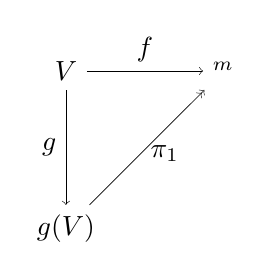
\begin{tikzpicture}
  %%% NODES
  \path (0,0) node(x) {$V$}
  (2,0) node(y) {$\RR^m$}
  (0,-2) node(z) {$g(V)$};
  %%% LINES
  \draw[very thin,->] (x) --node[above,midway] {$\vf{f}$} (y);
  \draw[very thin,->>] (z) --node[right,pos=0.45] {$\vf\pi_1$} (y);
  \draw[very thin,->] (x) --node[left,midway] {$\vf{g}$} (z);
\end{tikzpicture}

\end{document}